\section{Energy Saving Solution}
\label{sec:solution}

\definecolor{myblue}{RGB}{21,16,130} % RGB equivalent of #1f456e

\begin{figure}
    \centering
    \begin{tikzpicture}[
        scale=0.4, % Adjust this value if needed to fit the page width
        node distance = 1cm and 2cm,
        box/.style = {draw, fill=myblue, text=white, minimum width=2.5cm, minimum height=1.5cm, text width=2.5cm, align=center},
        arrow/.style = {-Stealth, thick}
    ]
    
    % Nodes
    \node[box] (tp) {\textbf{Traffic \\ Predictor}};
    \node[box, below=1cm of tp, xshift=0.5cm] (op) {\textbf{Overlap \\Predictor}};
    \node[box, right=1.5cm of tp] (da) {\textbf{Decision \\Making Entity}};
    \node[box, right=1.8cm of op] (dt) {\textbf{Digital \\Twin}};
    
    % Arrows
    \draw[arrow] ([xshift=-1.5cm, yshift=-1cm]tp.south west) to[out=0, in=180] (tp.west);
    \draw[arrow] ([xshift=-2.8cm, yshift=0.8cm]op.north west) to[out=0, in=180] (op.west);
    \draw[arrow] (tp.east) -- (da.west) node[midway, above] {\textbf{3}};
    \draw[arrow] (op.east) to[out=60, in=-90] (da.south);
    \draw[arrow] (dt.west) to[out=-120, in=-90] (op.south);
    \draw[arrow] (da.east) to[out=-45, in=45] (dt.north);
    \draw[arrow] (dt.south) -- ++(0,-1cm);

    % Labels
    \node[below=0.4cm of dt] {\textbf{Policy}};
    \node[left=0.35cm of tp, yshift=-0.4cm] {\textbf{1}};
    \node[left=0.55cm of op, yshift=0.3cm] {\textbf{2}};
    \node[below=0.5cm of da, xshift=-1cm] {\textbf{4}};
    \node[right=0.2cm of da, yshift=-0.7cm] {\textbf{5}};
    \node[left=0.9cm of dt, yshift=-0.7cm] {\textbf{6}};

    \end{tikzpicture}
    \caption{System architecture diagram}
    \label{fig:system-architecture}
    \end{figure}

The solution to address the two aspects of the problem discussed in the previous section comprises of several components as shown in \textcolor{blue}{CITE}. 
The data at each stage of the operational flow is indicated by numbers (1..6). 

The system is fed with the key performance indicators (KPI) data captured from the network (1) along with topology and configuration information (2). 
The former is consumed by the traffic predictor to determine if in the upcoming hours, the volume of the traffic changes by an amount necessary to relook at the current state of all the nodes. 
The topology and configuration data (2) is static information usually gathered from the Element Management System (EMS). 
The decision algorithm relies on the predicted traffic estimates (3) and the overlap predictions (5) to determine the state of the network, i.e., which nodes should be turned on and which should be off. 

However, at this stage, we need to make sure that such a decision is not detrimental to the performance of the network. 
Hence, it is run by the Digital Twin of the network to evaluate the “goodness” and if it passes a threshold, it is presented to the actual control unit, typically the EMS, for execution. 
Otherwise, we reevaluate the decision. Each of the components are complex systems and described in the following subsections.

Within the O-RAN framework, the application manifests as a rApp hosted in Non Realtime RIC and the decision is fed to xApp and SDNR. 
The data collection and cleaning is done at the edge cloud to take advantage of the distributed processing and avoid pushing large amounts of data to regional data centers.
Firstly, the E2 Nodes are configured by the Service Management and Orchestration (SMO) to report the data necessary via the O1 Interface. 
The functioning of the Non-RT RIC and SMO are tightly coupled, which enables the Non-RT RIC to retrieve the collected data through internal SMO communication. 

The rApp is data driven in the sense that it does not incorporate a rules-based logic but determines the rules which meet the target objective based on the input data and network configuration. 
The non-RT RIC, in particular, is designed to handle tasks that do not require immediate response. 
This makes it ideal for applications focused on long-term optimization and strategic planning, such as energy control. 

In our setup, the rApp receives input data from the Radio Database, Traffic Predictor, and Coverage Predictor, and sends a shutdown/bringup policy (a declarative statement across the A1 interface) to the Near-RT RIC. 
The Shutdown and Bringup of nodes is handled by a Traffic Steering xApp. 
The decision is made periodically, with a 1-hour prediction window and 15-minute slots, i.e., four predictions are made every window. 
The rApp is designed to be shared across multiple rApps and can import data from RF link simulators and drive tests through an external interface. 
A Dashboard for visualization of the Radio Mapping Database is also used as shown in the \textcolor{blue}{[CITE]}. \\

%\definecolor{mygrey}{RGB}{145,146,156}
\definecolor{mypurple}{RGB}{153,102,204}
\definecolor{myotherblue}{RGB}{0,191,255}
\definecolor{mygreen}{RGB}{144,238,144}
\definecolor{myyellow}{RGB}{255,215,0}
\definecolor{myorange}{RGB}{255,165,0}
\definecolor{myothergreen}{RGB}{35,79,30}
\definecolor{myred}{RGB}{255,127,80}
\definecolor{myindigo}{RGB}{100,110,230}

\begin{figure}
    \centering
    \begin{tikzpicture}[
        subox1/.style={draw, fill=myorange, minimum width=1.1cm, minimum height=0.7cm, font=\footnotesize},
        subox2/.style={draw, fill=myindigo, minimum width=0.55cm, minimum height=0.7cm, font=\footnotesize},
        subox3/.style={draw, fill=myred, minimum width=0.55cm, minimum height=0.7cm, font=\footnotesize},
        subox4/.style={draw, fill=myothergreen, minimum width=2.4cm, minimum height=0.4cm, font=\footnotesize},
        box1/.style={draw, fill=mygreen, minimum width=2.6cm, minimum height=1.5cm, font=\footnotesize},
        box2/.style={draw, fill=myyellow, minimum width=1.7cm, minimum height=1.5cm, font=\footnotesize},
        smallbox1/.style={draw, fill=mypurple, minimum width=0.85cm, minimum height=0.5cm, font=\footnotesize, rounded corners},
        smallbox2/.style={draw, fill=myotherblue, minimum width=0.85cm, minimum height=0.5cm, font=\footnotesize, rounded corners},
        smallbox3/.style={draw, fill=mygrey, minimum width=0.85cm, minimum height=0.5cm, font=\footnotesize, rounded corners},
        flatbox1/.style={draw, fill=myotherblue, minimum width=2cm, minimum height=0.25cm, font=\footnotesize},
        flatbox2/.style={draw, fill=myotherblue, minimum width=3.2cm, minimum height=0.25cm, font=\footnotesize},
        flatbox3/.style={draw, fill=mygrey, minimum width=3.2cm, minimum height=0.35cm, font=\footnotesize},
        bigbox1/.style={draw, fill=myotherblue, minimum width=0.8cm, minimum height=0.7cm, font=\footnotesize},
        bigbox2/.style={draw, fill=mygrey, minimum width=0.75cm, minimum height=0.7cm, font=\footnotesize},
        bigbox3/.style={draw, fill=mygrey, minimum width=4.45cm, minimum height=0.4cm, font=\footnotesize},
        hugebox/.style={draw, , fill=mygrey, minimum width=9cm, minimum height=0.75cm, font=\footnotesize},
        scale=0.4 % Adjust this value to fit in one or two columns
    ]
    
    % Base layer
    \node[hugebox, text=white] (ns3) {\textbf{\texttt{ns-3 (network simulator)}}};

    % Second layer
    \node[smallbox1, text=white, above left=0.2 and -1.5 of ns3] (sdnr) {\texttt{SDNR}};
    \node[flatbox1, text=white, above left=0.2 and -4.5 of ns3] (o1) {\texttt{O1-adapter}};
    \node[flatbox2, text=white, above right=0.2 and -3.2 of ns3] (e2) {\texttt{E2-adapter, USOI}};
    \node[flatbox3, text=white, above right=0.75 and -3.2 of ns3] (near-ric) {\textbf{\texttt{Near-RT RIC}}};
    
    % Third layer
    \node[bigbox1, text=white, above right=1.25 and -0.95 of ns3, align=center] (other-x) {\texttt{other} \\ \texttt{xApps}};
    \node[bigbox2, text=white, above right=1.25 and -2.27 of ns3, align=center] (kpi-x) {\textbf{\texttt{KPI-MON}} \\ \textbf{\texttt{xApp}}};
    \node[bigbox2, text=white, above right=1.25 and -3.15 of ns3, align=center] (ts-x) {\textbf{\texttt{TS}} \\ \textbf{\texttt{xApp}}};
    
    \node[bigbox3, text=white, above left=0.85 and -4.5 of ns3, align=center] (smo) {\textbf{\texttt{SMO}}};
    \node[bigbox3, text=white, above left=1.4 and -4.5 of ns3, align=center] (non-ric) {\textbf{\texttt{Non-RT RIC}}};

    % Fourth layer
    \node[box1, above left=0.15 and -2.6 of non-ric] (es) {};
    \node[box2, text=white, above left=0.15 and -4.45 of non-ric, align=center] (rapps) {\texttt{other} \\ \texttt{rApps}};
    
    % Super-Impose layer
    \node[subox1, text=white, above left=0.3 and -1.2 of non-ric, align=center] (dt) {\textbf{\texttt{DT}}};
    \node[subox2, text=white, above left=0.3 and -1.85 of non-ric, align=center] (cp) {\textbf{\texttt{CP}}};
    \node[subox3, text=white, above left=0.3 and -2.5 of non-ric, align=center] (tp) {\textbf{\texttt{TP}}};
    \node[subox4, text=white, above left=1.1 and -2.5 of non-ric, align=center] (dme) {\textbf{\texttt{DME}}};
    \node[smallbox1, text=white, above left=0.55 and -3.9 of ns3, align=center] (ves) {\texttt{VES} \\ \texttt{clctr}};
    
    % Arrows

    %\draw[-, line width=0.5mm] (sdnr.south) -- (ns3.north -| sdnr.south);
    %\draw[-, line width=0.5mm] (o1.south) -- (ns3.north -| o1.south);
    %\draw[-, line width=0.5mm] (e2.south) -- (ns3.north -| e2.south);
    %\draw[-, line width=0.5mm] (near-ric.south) -- (e2.north -| near-ric.south);
    %\draw[->, line width=0.5mm] (non-ric.south) -- (e2.north -| non-ric.south);
    
    % Text
    %\node[rotate=90, red, anchor=south, font=\tiny] at ($(es.west)+(-0.4,0)$) {Cell ON/OFF};
    \node[above=0.01 of es] {\small \textbf{\texttt{ES rApp}}};

    \end{tikzpicture}
    \caption{System Architecture Diagram}
    \label{fig:system-architecture}
\end{figure}
    

\begin{figure}[ht]
    \centering
    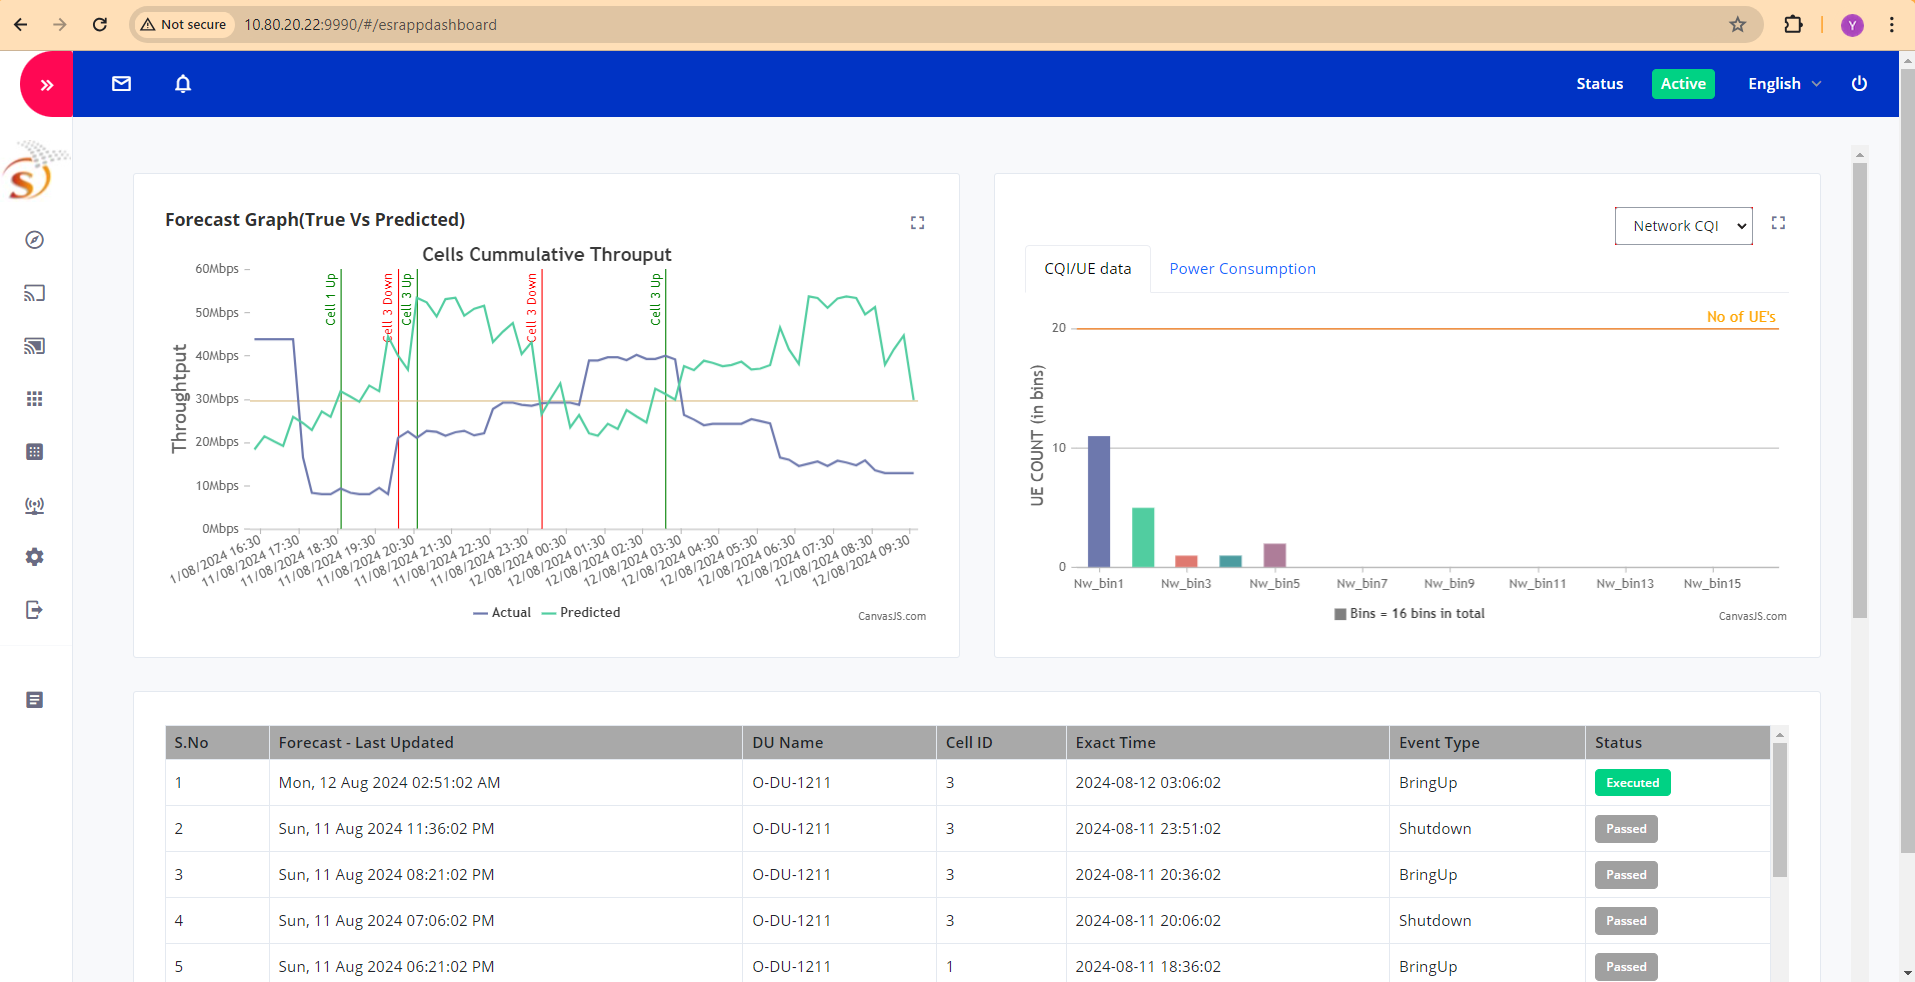
\includegraphics[width=0.4\textwidth]{/Users/pulakmehrotra/Desktop/SaankhyaLabs/es_oran_paper/acm_version_final/images/dashboard.png}
    \caption{ES rApp GUI}
    \label{fig:dashboard}
    \end{figure}

%Space-time partitioning: This is a technique used to divide data based on both spatial (location) and temporal (time) dimensions. In the context of the rApp, this could involve organizing Key Performance Indicators (KPIs) by specific geographical areas (cells, sectors, etc.) and time periods to better manage and analyze the data.
%Continuous time-based aggregation: This refers to the process of continuously collecting and summarizing data over time. Instead of analyzing data at discrete intervals, it is aggregated in a continuous manner, which allows for more fluid and accurate monitoring of KPIs.
%Group KPIs by time: This involves organizing the Key Performance Indicators (KPIs) into groups based on the time they were recorded. This helps in analyzing trends and patterns over specific time periods.
%The standalone application for an ESC node described in 2.2 is connected to the OpenSAS. This application indepen-dently senses the CBRS spectrum for any activity. If activityis detected, it sends IQ data to the model running insidethe OpenSAS for incumbent detection. The current imple-mentation is to detect incumbent (radar) in a 5G New Radio(NR) based CBRS network deployment. Additionally, the re-searchers could use this platform to experiment with theirown models for detecting signals of their interest throughthe ESC node in testbed environments.
%Network traffic prediction has always been a largely explored subject in networking, with a flurry of recent proposals ushered in by the recent development of machine and deep learning tools. Such deep learning-based algorithms have recently been explored to find potential representations of network traffic flows for all types of networks, including Internet, cellular, etc. We first categorize cellular traffic problems into two main types – temporal prediction problems and spatiotemporal prediction problems. Modelling the traffic flow through a node exclusively as a time series is an example of the temporal approach towards network traffic prediction [11]. High traffic on a given node in a cellular network often implies a high load on the other nearby nodes. Taking the traffic flow of nearby nodes and other external factors into consideration when modelling is known as the spatiotemporal approach to network traffic prediction. Spatiotemporal approaches are found to give slightly more accurate forecasts [12].
%Both types of problems can be formulated as supervised learning problems with a difference being in the form of feature representation. In the temporal approach, the collected traffic data can be represented as a univariate time series and the prediction for the values in the future time steps is based on the historical data of the past time steps. In [13], Clemente et Al used Naive Bayes classification and the Holt-Winters method to perform the temporal network forecasting in real time Clemenete et Al first performed systematic preprocessing to reduce bias by selecting the cells with less missing data occurrences, which was then selected to train the classifies to allocate the cells between predictable and non- predictable, taking into account previous traffic forecast error. 
%Building upon the temporal approach, Zhang et al. [14] presented a new technique for traffic forecasting that takes advantage of the tremendous capabilities of a deep convolutional neural network by treating traffic data as images. The spatial and temporal variability of cell traffic is well captured within the dimensions of the images. The experiments show that our proposed model is applicable and effective. Even with the ease of machine learning implementations, regression based models have been found to be fairly accurate, as proven by Yu et Al in [15]. In [15], Yu et Al applied a switching ARIMA model to learn the patterns present in traffic flow series, where the variability of duration is introduced and the sigmoid function describes the relation between the duration of the time series and the transition probability of the patterns. The MGCN-LSTM model, presented in [16] by Len et Al, was a spatial-temporal traffic prediction model which implemented a multi-graph convolutional network (MGCN) to capture spatial features, and a multi-channel long short-term memory (LSTM) to recognise the temporal patterns among short-term, daily, and weekly periodic data. The proposed model was found to greatly outperform commonly implemented algorithms such as ARIMA, LSTM and ConvLSTM.
%Hybrid models can handle a variety of data types and structures, making them ideal for diverse applications along with combining the best features of different methodologies. This very principle is proven by Kuber et Al in [17] which proposes a linear ensemble model composed of three separate sub-models. Each sub-model is used to predict the traffic load in terms of time, space and historical pattern respectively, handling one dimension particularly. Different methodologies such as time series analysis, linear regression and regression tree are applied to the sub-models, which is aggregated and found to perform comparable to a ResNet-based CNN model. Another approach for the same is highlighted in [18] Tian et Al. The approach involves analysing the chaotic property of network traffic by analyzing the chaos characteristics of the network data. [18] proposes a neural network optimization method based on efficient global search capability of quantum genetic algorithm and based on the study of artificial neural networks, wavelet transform theory and quantum genetic algorithm. The proposed quantum genetic artificial neural network model can predict the network traffic more accurately compared to a similarly implemented ARMA model.\\
	